 
\textbf{Ejemplo 8}\\
Supongamos que un inversionista desea adquirir la aceptación bancaria del ejemplo anterior, la cual figura con una tasa de registro del 30\% periódico 40 días vencido y con precio de registro $P_r =  97,65\%$ pero él también sabe que para adquirirla deberá pagar una comisión a un corredor de bolsa lo cual hará variar el precio que él debe pagar y también la rentabilidad que él pueda obtener. Supongamos que la comisión que cobra un corredor por la compra es del 0,475\% periodo 40 días periodo vencido ¿Cuál es el precio del comprador $P_c =  ? COP$ , que incluye la comisión del comisionista vendedor, el precio de registro y la comisión de bolsa del comprador. El punto de referencia es el precio de registro, $P_r$ ¿Cuál es la rentabilidad del inversionista, $i_c =? \%? $ periódica 40 días vencido, o $j=? $ nominal anual 40 dias vencido
%\newpage %USAR SOLO SI EL SOLUCIÓN QUEDA SOLO Y ES NECESARIO BAJARLO A LA SIGUIENTE PAGINA

\textbf{Solución.}
%La tabla ira centrada
\begin{center}
 \renewcommand{\arraystretch}{1.5}% Margenes de las celdas
 %Creación de la cuadricula de 3 columnas
 \begin{longtable}[H]{|p{0.33\linewidth}|p{0.33\linewidth}|p{0.33\linewidth}|}
 	%Creamos una linea horizontal
 	\hline
 	%Definimos el color de la primera fila
 	\rowcolor[HTML]{FFB183}
 	%%%%% INICIO ASIGNACIÓN FECHA FOCAL %%%%%%%
 	%%%%%%%%%% INICIO TITULO
 	%Lo que se hace aquí es mezclar las 3 columnas en una sola
 	\multicolumn{3}{|c|}{\cellcolor[HTML]{FFB183}\textbf{1. Asignación período focal}}                  \\ \hline
 	%%%%%%%%%% FIN TITULO
 	%%%%% INICIO DECLARACIÓN DE VARIABLES %%%%%%%
 	\multicolumn{3}{|c|}{$pf : 1 p (40 d) v. \textit{}$}                                                     \\ \hline
 	%%%%%%%%%% INICIO TITULO
 	%Lo que se hace aquí es mezclar las 3 columnas en una sola
 	\multicolumn{3}{|c|}{\cellcolor[HTML]{FFB183}\textbf{2. Declaración de variables}}                \\ \hline
 	%%%%%%%%%% FIN TITULO
 	%%%%%%%%%% INICIO SUBTITULO
 	\multicolumn{1}{|c|}{\cellcolor[HTML]{FFB183}\textbf{Valores monetarios}}    & 
 	\multicolumn{1}{|c|}{\cellcolor[HTML]{FFB183}\textbf{Valores no monetarios}} &
 	\multicolumn{1}{|c|}{\cellcolor[HTML]{FFB183}\textbf{Incógnitas}}  \\ \hline
 	%%%%%%%%%% FIN SUBTITULO
 	%%%%%%%%%% INICIO DE MATEMÁTICAS
 	%Cada & hace referencia al paso de la siguiente columna
 	& $i_c = 30\% - 0,475\% = 29,525\% \ p(40d)v$ & $V_r=?COP$                                     \\
 	& $P_r =  97,65  \% \textit{ COP}$ & $ P_c = COP$                                             \\
   
 	&$n = \frac{40}{365} \hspace{1mm} = 0,1096 \ p(40d)v  $ & $j = ? \ na(40d)v$\\ \hline
 	%%%%%%%%%% FIN DE MATEMÁTICAS
 	%%%%% FIN DECLARACIÓN DE VARIABLES
 	
 	\rowcolor[HTML]{FFB183}
 	\multicolumn{3}{|c|}{\cellcolor[HTML]{FFB183}\textbf{3. Diagrama de flujo de caja}}               \\ \hline
 	\multicolumn{3}{|c|}{ 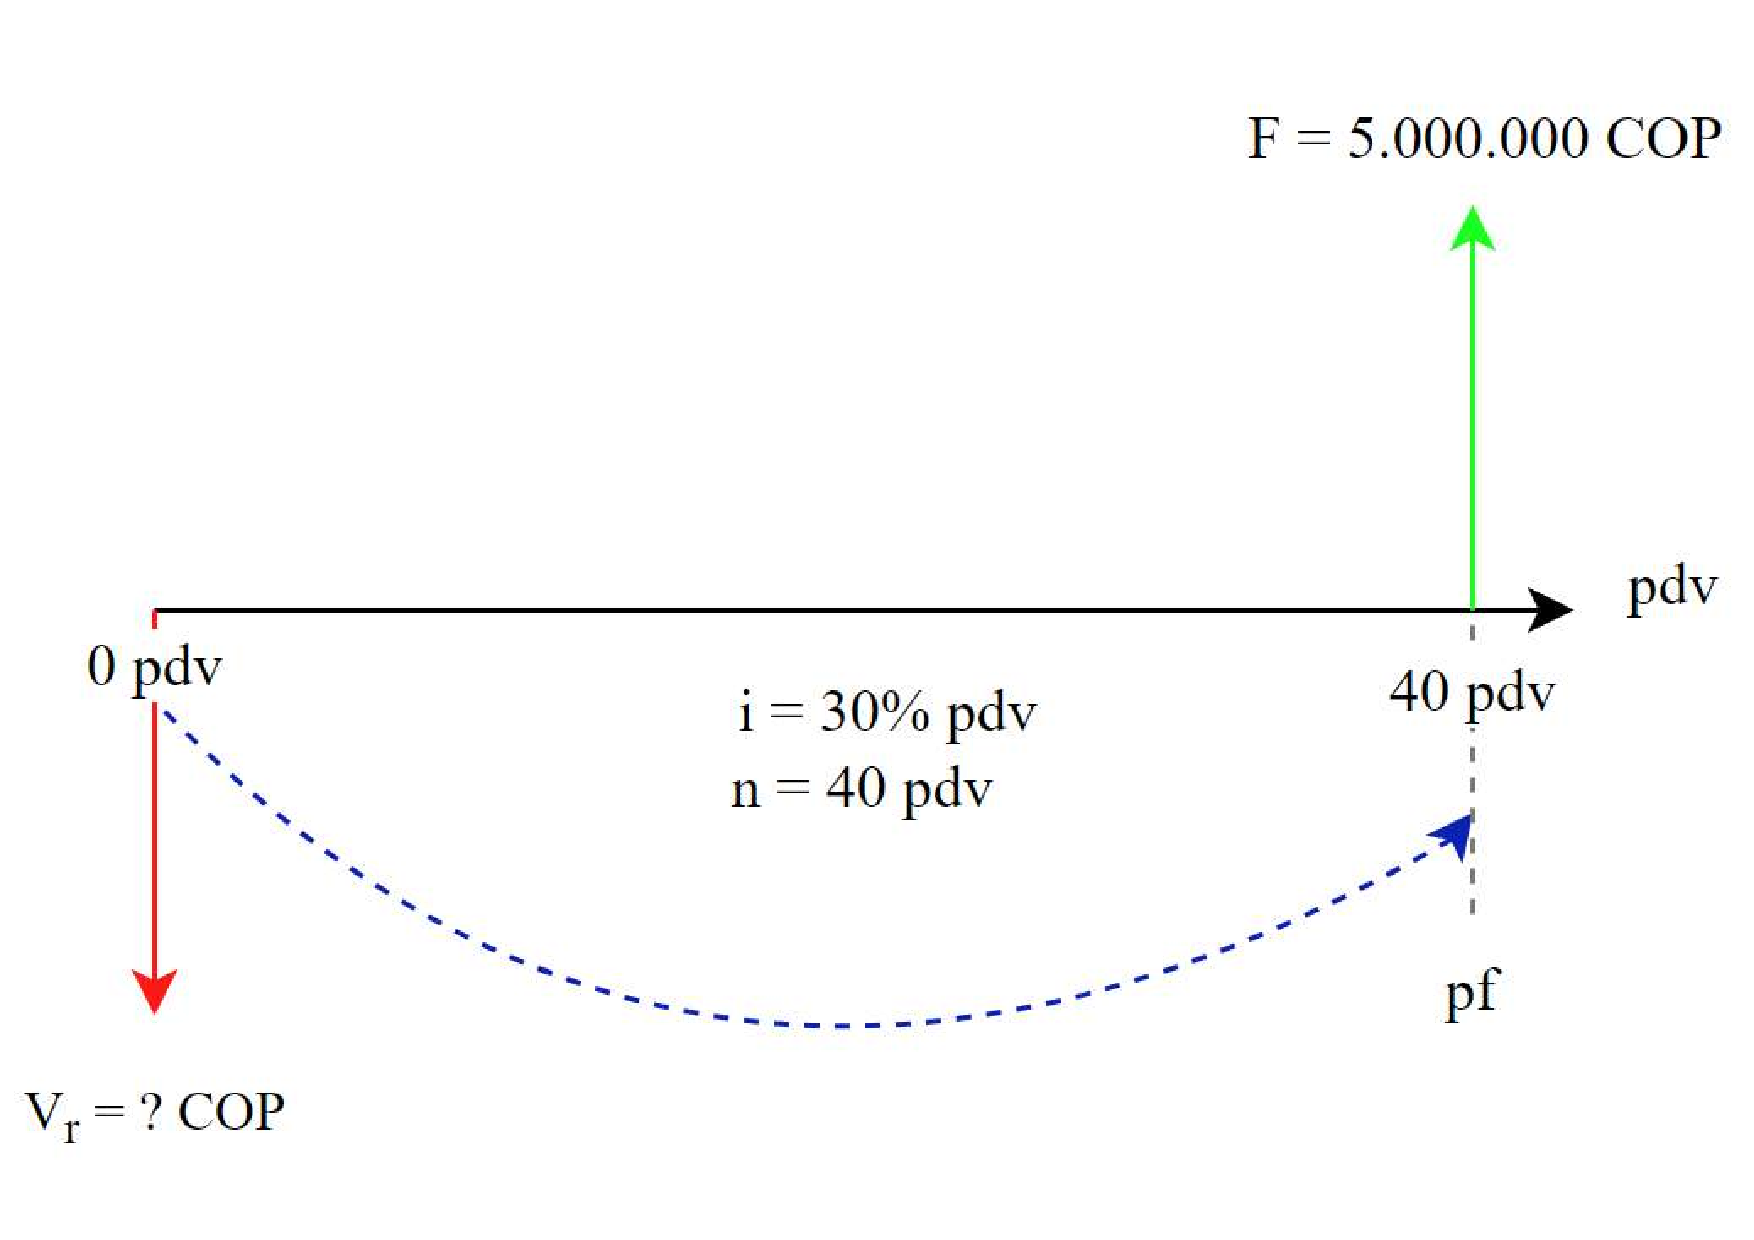
\includegraphics[trim=-5 -5 -5 -5 , scale=0.55, width=16.4 cm, height = 10.5 cm]{3_Capitulo/img/ejemplos/8/capitulo3ejercicio8.pdf} }  \\ \hline
 	%%%%% INICIO FLUJO DE CAJA
 	\rowcolor[HTML]{FFB183}
 	\multicolumn{3}{|c|}{\cellcolor[HTML]{FFB183}\textbf{4. Declaración de formulas}}                 \\ \hline
 	%Mezclamos 3 columnas y pondremos el dibujo
 	%%%%%%%%%%%%% INSERCIÓN DE LA IMAGEN
 	%Deberán descargar las imágenes respectivas del drive y pegarlas en la carpeta
 	%n_capitulo/img/ejemplos/1/capitulo1ejemplo1.pdf  (el /1/ es el numero del ejemplo)
 	\multicolumn{3}{|c|}{ $P = F(1 + i)^(-n) $ Valor presente }  \\
 	\multicolumn{3}{|c|}{ $(1 + ij)^m = (1 + i)^m $ Equivalencia de tasas }
 	\\ \hline
 	%%%%%%%%%%%%% FIN INSERCIÓN DE IMAGEN
 	%%%%%FIN FLUJO DE CAJA
 	
 	
 	%%%%%% INICIO DESARROLLO MATEMÁTICO
 	\rowcolor[HTML]{FFB183}
 	%%%%%%%%%%INICIO TITULO
 	\multicolumn{3}{|c|}{\cellcolor[HTML]{FFB183}\textbf{5. Desarrollo matemático}}                   \\ \hline
 	%%%%%%%%%% FIN TITULO
 	%%%%%%%%%% INICIO MATEMÁTICAS
 	\multicolumn{3}{|C{\linewidth}|}{
 		$P_c =  100 COP(1 + 0,29525)\frac{-40}{365} = 97,204 \%COP$ Ecuación de equivalencia
 		
 		$V_r = 0,972047( 5{.}000{.}000 COP) =  4{.}860{.}245 COP$
 		
 		$P_c - V_r =  4{.}860{.}235 COP -  4{.}858{.}285 COP = 1{.}950 COP$
 	}   \\   
 	\multicolumn{3}{|p{\linewidth}|}{$ \ \ Calculamos i$}  \\
 	\multicolumn{3}{|C{\linewidth}|}{
 		$(1 + j) = (1 + 0.3)^{\frac{365}{40}}$ 
 		
 		$j = (1 + 0.3)^{\frac{365}{40}} - 1$
 		
 		$j = 1,0743151 - 1$
 		
 		$j = 0,0743151 \textit{ na(40d)v}$
 	}
 	\\ \hline
 	
 	%%%%%%%%%% FIN MATEMÁTICAS
 	%%%%%% FIN DESARROLLO MATEMÁTICO
 	%%%%%% INICIO RESPUESTA
 	\rowcolor[HTML]{FFB183}
 	%%%%%%%%%%INICIO TITULO
 	\multicolumn{3}{|c|}{\cellcolor[HTML]{FFB183}\textbf{6. Respuesta}}                               \\ \hline
 	%%%%%%%%%% FIN TITULO
 	%%%%%%%%%% INICIO RESPUESTA MATEMÁTICA
 	\multicolumn{3}{|C{\textwidth}|}{
 		$V_r =  4{.}860{.}245 COP$
 		$j = 7,43151 nadv$
 	}                                                                                                 \\ \hline
 	
 	
 	%%%%%%%%%% FIN MATEMÁTICAS
 	%%%%%% FIN RESPUESTA
 \end{longtable}
 
 %Se crean dos lineas en blanco para que no quede el siguiente texto tan pegado
 %\newline \newline %USARLO SI CREES QUE ES NECESARIO
\end{center}